\begin{center}\large\textbf{Readings: Chapter 4 - 4.1-4.4, 4.6-4.8 (ok to skip Poisson Distribution), 4.9-4.10, 4.12, 4.14}\\
\normalsize \end{center}
\large ~\hrulefill
~\\
\normalsize \\

Recall:  Our goal is to conduct inference.  In order to do this, we need a firm understanding of probability.\\~\\
\textbf{Interpretation of Probability}\\
\bi
\item \underbar{~~~~~~~~~~~~~~~~~~~~~~~~~~~~~~~~~~~~~~~~~~~~~~~~~~~~} of an outcome in repeated experiment = \# of times outcome observed/\# of times experiment was repeated
\bi
\item Ex: the chance of rolling snake eyes ($(1,1)$) on two fair dice
\item Ex: the chance of getting a head on a flipped coin
\ei
\ei
Probability and Inference
\bi
\item Ex:  We want to see if a coin is fair.  If we formulate the research question in terms of parameters, we want to test the \underline{hypothesis}:\\~\\~\\~\\~\\~\\
Suppose the coin is tossed $n=10$ times and yields $y=10$ heads. 
\bi
\item If hypothesis is true, how likely is the observed event?\\
\item With 10/10 heads, reasonable to conclude coin not fair.  What about 9/10 heads? 7/10 heads?\\
\item To make a decision, need to know \underbar{~~~~~~~~~~~~~~~~~~~~~~~~~~~~~~~~~~~~~~~~~~~~~~}
\ei
\ei
\begin{center}
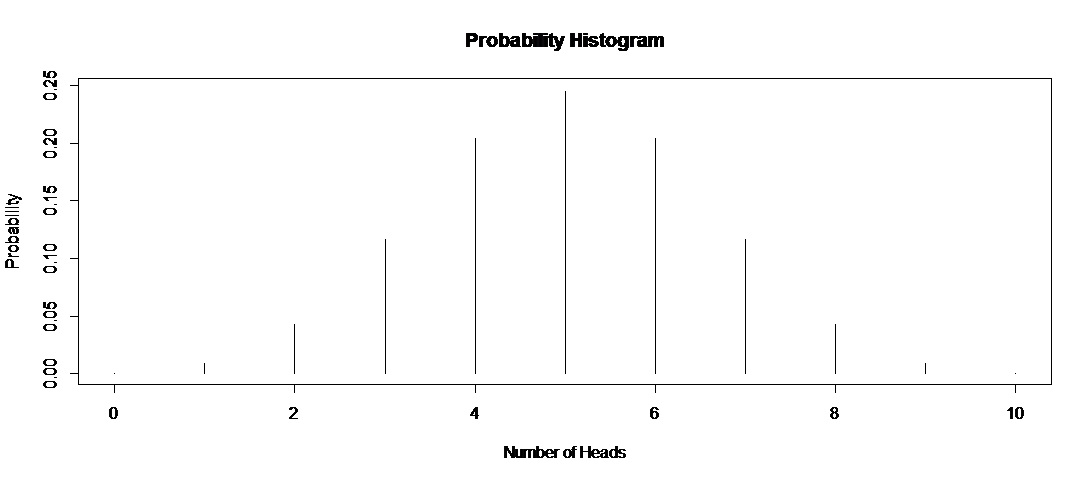
\includegraphics[scale=0.35]{chapter4/binomialprobhist.jpg}
\end{center}
The above plot gives the probability of observing a given number of heads from a fair coin in 10 tosses.  \\~\\~\\~\\~\\

\huge Sets and Sample Spaces\\ \normalsize
A probability model is a mathematical representation of a random phenomenon. Defined by its
\bi
\item %Sample space 
\item %Events within the sample space 
\item %Probabilities associated with each event.
\ei
\textbf{Definitions:}
\bi
\item \underbar{~~~~~~~~~~~~~~~~~~~~~~~}: A collection of \textbf{elements}, $a_1,a_2,\ldots$\\
\item \underbar{~~~~~~~~~~~~~~~~~~~~~~~~~~~~~~~~~~~~~~~~~~~}: the set of all outcomes under consideration\\
\item \underbar{~~~~~~~~~~~~~~~~~~~~~~~}: Each possible distinct result of a random process (experiment)\\
\item $A$ is a \underbar{~~~~~~~~~~~~~~~~~~~~~~~~~~} of $B$ if every element of $A$ belongs to $B$ ($A \subset B$)\\
\item \underbar{~~~~~~~~~~~~~~~~~~~~~~~}: A collection of outcomes (a subset of \textbf{S})\\
\ei

\textbf{Sample Space examples:}\\
Define the sample space \textbf{S} for each situation below.\\
Of the parts manufactured today, randomly select and measure the thickness of \textbf{a single part}.  \\~\\~\\
It is known that the thickness must be between 10 and 11 mm.   \\~\\~\\
It is known that the thickness has only three values (low, medium or high). \\~\\~\\
Experiment asks, does the part thickness meet specifications?\\~\\~\\
Now two parts are randomly selected and measured.\\~\\~\\
Do the 2 parts conform to specifications? \\~\\~\\
Number of conforming parts from the two is measured.\\~\\~\\
Now, parts are randomly selected until a non-conforming part is found.\\~\\~\\~\\~\\

\textbf{More Set definitions:}
\bi
\item \underbar{~~~~~~~~~~~~~~~~~~~~~~~~~~} ($A \cup B$): the set of all points in $A$ or $B$ (including both)\\
\item \underbar{~~~~~~~~~~~~~~~~~~~~~~~~~~} ($A \cap B$): the set of all points in both $A$ and $B$\\
\item \underbar{~~~~~~~~~~~~~~~~~~~~~~~~~~} of $A$ ($\bar{A}$ or $A^c$): contains elements in $S$ but not in $A$\\
\item $A$ and $B$ are \underbar{~~~~~~~~~~~~~~~~~~~~~~~~~~} or \underbar{~~~~~~~~~~~~~~~~~~~~~~~~~~} if $A\cap B = \emptyset$.\\~\\~\\
\ei

\textbf{Gender of Children - Discrete Example}: - A family has two children of different ages.  Consider the possible genders of these children. Let a pair $FM$ denote the element in which the younger child is female and the older is male.
\be
\item Sample Space: $S=\{~~~~~~~~~~~~~~~~~~~~~~~~~~~~~~~~\}$
\item Let $A$ be the event in which both children are males, $B$ the event in which there is at least one male, and $C$ the event containing no males.\\
List the elements of
    \bi
    \item $A=\{~~~~~~~~~~~~~~~~~~~~~~~~~\}$ $~~~~~~~~$ $A\cup C =\{~~~~~~~~~~~~~~~~~~~~~~~~~\}$\\
    \item $B=\{~~~~~~~~~~~~~~~~~~~~~~~~~\}$ $~~~~~~~~$ $\bar{A} =\{~~~~~~~~~~~~~~~~~~~~~~~~~\}$\\
    \item $C=\{~~~~~~~~~~~~~~~~~~~~~~~~~\}$ $~~~~~~~~$ $A \cup B=\{~~~~~~~~~~~~~~~~~~~~~~~~~\}$\\
    \item $A\cap C =\{~~~~~~~~~~~~~~~~~~~~~~~~~\}$ $~~~$ $B \cup \bar{A}=\{~~~~~~~~~~~~~~~~~~~~~~~~~\}$
    \ei
\ee

\newpage

\huge Relating Set Theory to Probability \\\normalsize
\bi
\item An \underbar{~~~~~~~~~~~~~~~~~~~~~~~~~~} is any process that can be repeated (theoretically) and has a well-defined set of possible outcomes (sample space)\\
\item An event corresponds to \underbar{~~~~~~~~~~~~~~~~~~~~~~~~~~~~~~~~~~~~~~~~~~~~~~~~~~~~~~~~~~~~~~~~~~}
\item The Probability of the event is the likelihood or chance that a particular outcome or event from a random experiment will occur.  We write 
$$P(A) = \mbox{Probability the event A occurs}$$
\item Probabilities are numbers between \underbar{~~~~~~~~~~~~~~~~~~~~~~~~~~~~~~~~~~~~~~~~~~~~~~~~~~}
\item May be written as proportion (0.15), percent (15\%), or a fraction (3/20).\\
\item P(Event)=1 implies \underbar{~~~~~~~~~~~~~~~~~~~~~~~~~~~~~~~~~~~~~~~~~~~~~~~~~~~~~~~~~~~~~~~~~~~~~~~~~~~~}\\
\item P(Event)=0 implies \underbar{~~~~~~~~~~~~~~~~~~~~~~~~~~~~~~~~~~~~~~~~~~~~~~~~~~~~~~~~~~~~~~~~~~~~~~~~~~~~}\\
\ei

\large\textbf{Simplified axioms of probability}\normalsize\\
\bi
\item The probability of an event, $P(A)$, a function, must satisfy:\\~\\~\\
\underbar{~~~~~~~~~~~~~~~~~~~~~~~~~~~~~~~~~~~~~~~~~~~~~~~~~~~~~~~~~~~~~~~~~~~~~}\\~\\~\\
\underbar{~~~~~~~~~~~~~~~~~~~~~~~~~~~~~~~~~~~~~~~~~~~~~~~~~~~~~~~~~~~~~~~~~~~~~}\\~\\
If A and B are disjoint (mutually exclusive) then\\~\\~\\
\underbar{~~~~~~~~~~~~~~~~~~~~~~~~~~~~~~~~~~~~~~~~~~~~~~~~~~~~~~~~~~~~~~~~~~~~~}\\
\ei

\textbf{Probability example (Recall Gender of Children ex)} - The sample space for this experiment was
$$\mbox{\textbf{S}}=\left\{MM, MF, FM, FF\right\}$$
\be
\item What would be reasonable probabilities for each outcome in $S$?\\
\item For A, B, and C, defined earlier, find $P(A)$, $P(B)$, $P(C)$, $P(A\cup C)$, and $P(S)$
\ee

\newpage

\huge\textbf{Conditional Probability, Independence, and Other Probability Rules}\normalsize\\~\\
Often we will have knowledge of one event's occurrence.  How does that change the probability of another event?\\~\\

For example, the probability of getting a 1 in the toss of a six-sided die is \underline{~~~~~~~~~~~~~~~}.\\~\\
If we know that an odd number has fallen, then the probability of occurrence of a 1 is \underline{~~~~~~~~~~~~~~}.\\~\\~\\
The \underbar{~~~~~~~~~~~~~~~~~~~~~~~~~~~~~~~~~~~~~~~~~~~~~~~~~~~} of an event $A$ given that an event $B$ has occurred is equal to\\~\\~\\~\\~\\~\\
provided $P(B)>0$.\\~\\

\textbf{Independent Events}\\ 
Two events and are said to be \underbar{~~~~~~~~~~~~~~~~~~~~~~~~~~~~~~~~~~~~~~} if and only if \textbf{any} one of the following 3 conditions hold:
\begin{eqnarray*}
P(A|B) &=& P(A)\\
P(B|A) &=& P(B)\\
P(A \cap B) &=& P(A)P(B).
\end{eqnarray*}
~\\Otherwise, the events are said to be \underbar{~~~~~~~~~~~~~~~~~~~~~~~~~~~~~~~~~~~~~~~~~~~~~~~~~~~~~}\\~\\~\\


\textbf{Independence Examples}
\bi
\item Consider again the ``Gender of Children" example.  Let $A$ be the event that the younger child is female, and $B$ be the event that the older child is male.  Are $A$ and $B$ dependent?

\newpage

\item (Credit Card Example) - The proportion of NCSU students with a VISA card is 0.48, the proportion with a MasterCard is 0.64, the proportion with both is 0.35.
\be
\item Calculate the conditional probability that a randomly sampled student has a VISA given he/she has a MasterCard.\\~\\~\\~\\~\\
\item Are the events `having a VISA' and `having a MasterCard' independent?\\~\\~\\~\\~\\
\ee
\ei

\textbf{Laws of Probability}\\
Sometimes probabilities of events can be obtained by using multiplicative and additive rules.\\~\\
\textbf{\underbar{~~~~~~~~~~~~~~~~~~~~~~~~~~~~~~~~~~~~~~~~~~~~~~~~~~~~~~~~}:}
\begin{center}
\fbox{$P(A \cap B) = P(B|A)P(A) = P(A|B)P(B)$}
\end{center}
~\\
Notice that if $A$ and $B$ are \underbar{~~~~~~~~~~~~~~~~~~~~~~~~~~~~~~~~~~~~~~}, then\\
\begin{center}
\fbox{ $P(A\cap B) = P(A)P(B)$}
\end{center}
~\\~\\

\textbf{Using the Multiplicative Law}\\
(Urn Example) - An urn contains 10 marbles, 4 are red (R) and 6 are black (B).
\be
\item If 2 are randomly chosen from the urn, what is the probability that both are black?\\~\\~\\~\\
\item If 1 is randomly chosen, then replaced, and then another randomly chosen (making the selections independent events), what is the probability of selecting a red then a black?\\~\\~\\~\\
\item Flip a fair coin 3 times, find the probability of observing 3 heads (HHH) assuming independent flips.
\ee

\newpage

\textbf{\underbar{~~~~~~~~~~~~~~~~~~~~~~~~~~~~~~~~~~~~~~~~~~~~~~~~~~~~~~~~~~~~~~~~~~~~~~~}:}\\
\begin{center}
\fbox{$P(A\cup B) = P(A) + P(B) - P(A \cap B)$}
\end{center}
Recall 3rd axiom: if $A$ and $B$ are disjoint, then $P(A \cup B) = P(A) + P(B)$.\\
\begin{center}
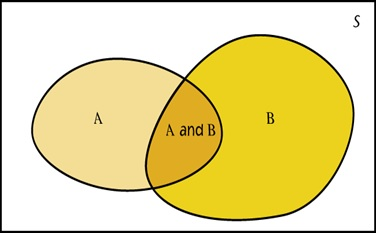
\includegraphics[angle=0,width=2in,totalheight=1in]{chapter4/AandB.jpg}
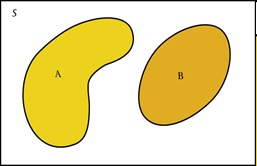
\includegraphics[angle=0,width=2in,totalheight=1in]{chapter4/AandB2.jpg}
\end{center}
~\\

\textbf{Using the Additive Law}
\bi
\item (Credit Card Example) - The proportion of NCSU students with a VISA card is 0.48, the proportion with a MasterCard is 0.64, the proportion with both is 0.35.  \\
Find the probability that a randomly sampled student has a VISA or MasterCard (or both).\\~\\~\\~\\
\item (Axiom Example) - Can $A$ and $B$ be mutually exclusive if $P(A)=0.4$ and $P(B)=0.7$? What if $P(B)=0.3$?\\~\\~\\~\\~\\
\ei

\textbf{\underbar{~~~~~~~~~~~~~~~~~~~~~~~~~~~~~~~~~~~~~~~~~~~~~}}:\\
A special case of additive law is obtained by taking $B = A^{c}$, then
\begin{center}
\fbox{$P(A) + P(A^{c}) = 1$ implies $P(A)=1-P(A^{c})$}
\end{center}
~\\
Ex: In 17th century De M'er'e asked Pascal, which is more likely:\\
\indent A: rolling at least one six in four throws of a single dice, or\\
\indent B: rolling at least one double six in 24 throws of a pair of dice?\\
Find $P(A)$ and $P(B)$.\\~\\~\\~\\~\\~\\~\\


(See example 4.1 on page 149.)
	
